\subsection{Multi-Path (Two-Path) CTLE}
\label{sec:multipath_ctle}

\begin{figure}[H]
    \centering
    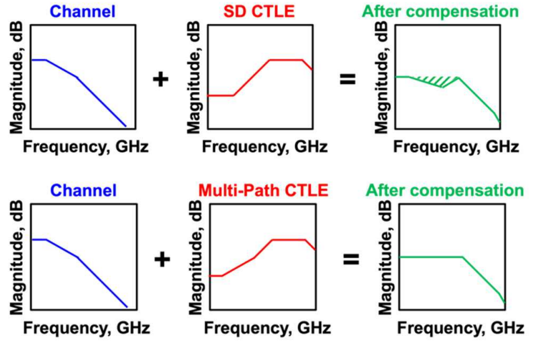
\includegraphics[width=.7\textwidth]{img/CTLE_img/idea of multipath_mid compensation.png}
    \caption{Channel equalization comparison: Multi-path CTLE provides flatter compensation across the entire bandwidth compared to SD-CTLE. \cite{11223232}}
    \label{fig:multipath_compensation}
\end{figure}

The Multi-Path CTLE, specifically the Two-Path implementation, addresses the limitations of single-path equalizers by adding a secondary signal path that introduces additional pole-zero pairs. As shown in Figure~\ref{fig:multipath_compensation}, while conventional SD-CTLE primarily boosts high-frequency components, it often leaves mid-band frequencies under-compensated. The multi-path architecture effectively compensates for these mid-band channel losses that cannot be adequately corrected by conventional single-path CTLEs, flattening the overall frequency response across the entire Nyquist bandwidth and achieving more uniform compensation from DC to the Nyquist frequency.


\subsubsection*{Architecture and Operating Principle}
\label{subsec:multipath_architecture}

\begin{figure}[H]
    \centering
    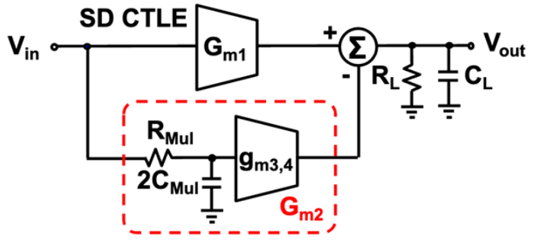
\includegraphics[width=0.35\textwidth]{img/CTLE_img/multipath block diagram.png}
    \caption{Block diagram of the two-path CTLE.\cite{11223232}}
    \label{fig:multipath_block_diagram}
\end{figure}

The Two-Path CTLE concept, illustrated in Figure~\ref{fig:multipath_block_diagram}, combines a primary SD-CTLE path ($G_{m1}$) with a secondary compensating path ($G_{m2}$) through a summing node. The secondary path, implemented with transconductance $G_{m3,4}$ and RC network $R_{Mul}$-$C_{Mul}$, introduces frequency-dependent characteristics that complement the primary path's response.

\begin{figure}[H]
    \centering
    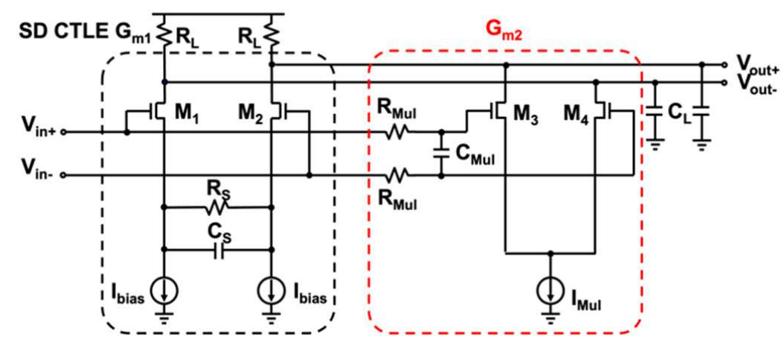
\includegraphics[width=0.65\textwidth]{img/CTLE_img/multipath schematic.png}
    \caption{Two-path CTLE circuit implementation with primary SD-CTLE and secondary compensating path. \cite{11223232}}
    \label{fig:multipath_schematic}
\end{figure}

The circuit implementation, shown in Figure~\ref{fig:multipath_schematic}, realizes the block diagram with transistors $M_1$-$M_2$ forming the primary SD-CTLE path, while $M_3$-$M_4$ with $R_{Mul}$ and $C_{Mul}$ create the secondary path. The fundamental principle is that "Multi-path CTLE adds another pole-zero path that fixes mid-band loss and flattens the overall response when a single CTLE can't compensate the channel shape."

\subsubsection*{Frequency Response Analysis}
\label{subsec:multipath_freq_response}

\begin{figure}[H]
    \centering
    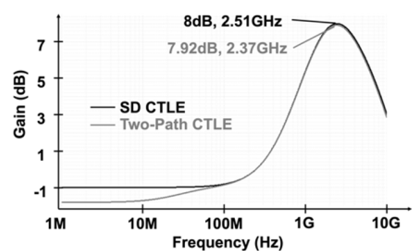
\includegraphics[width=0.4\textwidth]{img/CTLE_img/multipath real response.png}
    \caption{Frequency response comparison of two-path CTLE in 180nm technology.}
    \label{fig:multipath_real_response}
\end{figure}

The transfer function for the Two-Path CTLE is:

\[
H_2(s) \simeq -\left( \frac{g_{m1,2}}{1 + \frac{g_{m1,2}R_s}{2}} - g_{m3,4} \right) R_L \cdot \frac{\left(1 + \frac{s}{\omega_z}\right)\left(1 + \frac{s}{\omega_{z_{Mul}}}\right)}{\left(1 + \frac{s}{\omega_{p1}}\right)\left(1 + \frac{s}{\omega_{p2}}\right)\left(1 + \frac{s}{\omega_{p_{Mul}}}\right)}
\]

The additional pole-zero pair introduced by the secondary path is characterized by:

\[
\begin{aligned}
\omega_{p_{Mul}} &= \frac{1}{2R_{Mul}C_{Mul}}, &\quad
\omega_{z_{Mul}} &= \frac{g_{m1,2} - g_{m3,4}\left(1 + \frac{g_{m1,2}R_s}{2}\right)}{2g_{m1,2}R_{Mul}C_{Mul}}, &\quad
G_{m2} &= \frac{g_{m3,4}}{1 + s2R_{Mul}C_{Mul}}
\end{aligned}
\]

The DC gain of the composite system is:

\[
\text{DC Gain} \approx \left( \frac{g_{m1,2}}{1 + \frac{g_{m1,2}R_s}{2}} - g_{m3,4} \right) R_L
\]

 The additional zero $\omega_{z_{Mul}}$ introduced by the secondary path provides the critical mid-frequency compensation needed to flatten the overall response.

\subsubsection*{Design Knobs and Tunability}
\label{subsec:multipath_design_knobs}

\subsubsection*{Effect of Resistance $R_{Mul}$}
\label{subsubsec:effect_rmul}

\begin{figure}[H]
    \centering
    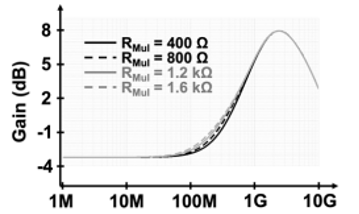
\includegraphics[width=0.4\textwidth]{img/CTLE_img/multipath effect of Rmul.png}
    \caption{Frequency response variation with increasing $R_{Mul}$ in 180nm technology.}
    \label{fig:effect_rmul}
\end{figure}

The resistance $R_{Mul}$ controls the pole frequency $\omega_{p_{Mul}} = \frac{1}{2R_{Mul}C_{Mul}}$ of the secondary path. As shown in Figure~\ref{fig:effect_rmul}:

\begin{itemize}
    \item Increasing $R_{Mul}$ from 400 $\Omega$ to 1.6 k$\Omega$ reduces $\omega_{p_{Mul}}$, shifting the secondary path's influence to lower frequencies.
    \item Larger $R_{Mul}$ values enhance mid-band compensation but may reduce high-frequency peaking.
    \item Optimal $R_{Mul}$ depends on the specific channel's mid-band loss characteristics.
\end{itemize}

\subsubsection*{Effect of Capacitance $C_{Mul}$}
\label{subsubsec:effect_cmul}

\begin{figure}[H]
    \centering
    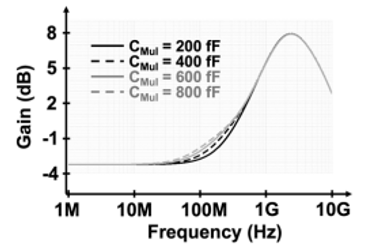
\includegraphics[width=0.4\textwidth]{img/CTLE_img/multipath effect of Cmul.png}
    \caption{Frequency response variation with increasing $C_{Mul}$ in 180nm technology.}
    \label{fig:effect_cmul}
\end{figure}

The capacitance $C_{Mul}$ works with $R_{Mul}$ to set $\omega_{p_{Mul}}$. As shown in Figure~\ref{fig:effect_cmul}:

\begin{itemize}
    \item Increasing $C_{Mul}$ from 200 fF to 800 fF lowers $\omega_{p_{Mul}}$, similar to increasing $R_{Mul}$.
    \item Larger $C_{Mul}$ values provide stronger mid-band compensation at the cost of area consumption.
    \item $C_{Mul}$ offers additional tuning freedom beyond what $R_{Mul}$ alone can provide.
\end{itemize}

\subsubsection*{Effect of Transistor Width $W_{3,4}$}
\label{subsubsec:effect_w34}

\begin{figure}[H]
    \centering
    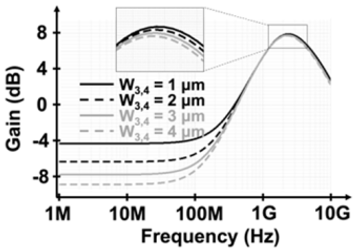
\includegraphics[width=0.4\textwidth]{img/CTLE_img/multipath effect of w.png}
    \caption{Frequency response variation with increasing $W_{3,4}$ in 180nm technology.}
    \label{fig:effect_w34}
\end{figure}

The transistor widths $W_{3,4}$ control $g_{m3,4}$ of the secondary path, affecting both $\omega_{z_{Mul}}$ and the overall gain balance. As shown in Figure~\ref{fig:effect_w34}:

\begin{itemize}
    \item Increasing $W_{3,4}$ boosts $g_{m3,4}$, strengthening the secondary path's contribution.
    \item Larger $W_{3,4}$ enhances mid-band compensation but as a secondary effect it reduces overall peaking.
    \item The zero location $\omega_{z_{Mul}}$ depends on the ratio between $g_{m1,2}$ and $g_{m3,4}$.
\end{itemize}

\subsubsection*{Design Trade-offs}
\label{subsec:multipath_tradeoffs}

\begin{table}[H]
\centering
\caption{Two-Path CTLE Design Trade-offs}
\label{tab:multipath_tradeoffs}
\begin{tabular}{ >{\raggedright\arraybackslash}p{0.15\textwidth} 
                 >{\raggedright\arraybackslash}p{0.23\textwidth} 
                 >{\raggedright\arraybackslash}p{0.25\textwidth} 
                 >{\raggedright\arraybackslash}p{0.30\textwidth} }
\toprule
\textbf{Parameter} & \textbf{Benefit} & \textbf{Risk} & \textbf{Design Guideline} \\
\midrule
$R_{Mul}$ & Controls $\omega_{p_{Mul}}$, mid-band tuning & Reduced peaking if too large & Optimize for channel mid-loss \\
$C_{Mul}$ & Adjusts $\omega_{p_{Mul}}$, area-efficient tuning & Parasitic sensitivity & Co-design with $R_{Mul}$ \\
$W_{3,4}$ & Sets $g_{m3,4}$, affects $\omega_{z_{Mul}}$ & May cancel primary path gain & Balance with $g_{m1,2}$ \\
$g_{m3,4}$ & Determines secondary path strength & Complex gain interaction & Target 20-40\% of $g_{m1,2}$ \\
Path Balance & Flattened response, better ISI reduction & Requires careful optimization & Simulate with target channel \\
\bottomrule
\end{tabular}
\end{table}

\textbf{Advantages over Single-Path SD-CTLE:}
\begin{itemize}
    \item \textbf{Mid-Band Loss Compensation}: Specifically addresses frequency regions where single-path CTLEs under-compensate.
    \item \textbf{Flatter Overall Response}: Achieves more uniform gain from DC to Nyquist frequency.
    \item \textbf{Enhanced Equalization Flexibility}: Multiple tuning parameters adapt to complex channel profiles.
    \item \textbf{Reduced Residual ISI}: Better elimination of both pre-cursor and post-cursor interference.
\end{itemize}

\newpage